\documentclass[11pt,a4paper]{jsarticle}



%%%%%%%%%%%%%%%%%%%%%%%%%

% Packages

%%%%%%%%%%%%%%%%%%%%%%%%%

\usepackage{amsmath}  % 環境
\usepackage{amssymb}  % 記号
\usepackage{amsfonts} % 特殊文字

\usepackage{ascmac}

\usepackage{ulem}

\usepackage{lmodern}

\usepackage{bm}

\usepackage{mathtools, centernot, physics}

\usepackage{enumerate}

% \usepackage{graphicx}

\usepackage[dvipdfmx]{graphicx}

\usepackage{comment} % 複数行をコメントアウトする

\usepackage{url}

\usepackage{array, booktabs, multirow, makecell} % tabular関連

% \usepackage{romannum} % ローマ数字

% \usepackage{xcolor}

\usepackage[dvipdfmx, dvipsnames]{xcolor}

\usepackage{setspace}

\usepackage{float}



%%%%%%%%%%%%%%%%%%%%%%%%%

% Format

%%%%%%%%%%%%%%%%%%%%%%%%%

\setlength{\textwidth}{\fullwidth}

\setlength{\textheight}{40\baselineskip}

\addtolength{\textheight}{\topskip}

\setlength{\voffset}{-0.2in}

\setlength{\topmargin}{0pt}

\setlength{\headheight}{0pt}

\setlength{\headsep}{0pt}



%%%%%%%%%%%%%%%%%%%%%%%%%

% Definitions

%%%%%%%%%%%%%%%%%%%%%%%%%

\newcommand{\alert}[1]{\textbf{\textcolor{red}{#1}}}

\newcommand{\rainn}{\textcolor{blue}{\uline{\ \ \ \ }}}

\newcommand{\sizi}[1]{\textcolor{OliveGreen}{\lbrack #1\rbrack}}



	

\begin{document}

\section{目的}
トランジスタの静特性(直流特性)を測定し、その入出力インピーダンスのふるまい、増幅動作を理解する。

\section{原理}
バイポーラトランジスタは、ベース(B)、コレクタ(C)、エミッタ(E)の3端子を有する半導体素子であり、
小さな入力信号によって大きな出力信号を制御できることから、増幅素子として広く用いられている。
npn形バイポーラトランジスタでは、ベースーエミッタ間接合が順方向バイアスされ、
コレクタ－ベース間接合が逆方向バイアスされた状態で動作する。

ベース層は非常に薄く形成されているため、エミッタからベースへ注入された電子の大部分はベース中で再結合することなく
コレクタへ到達する。このため、コレクタ電流$I_C$は主としてベース－エミッタ間電圧$V_{BE}$によって制御される。
一方、ベース電流$I_B$は比較的小さく、コレクタ電流との比

\begin{equation}
h_{FE}=\frac{I_C}{I_B}
\end{equation}

を直流電流増幅率という。$h_{FE}$が大きいほど、小さなベース電流によって大きなコレクタ電流を制御することができる。

また，トランジスタを微小信号に対して線形素子として扱う際には、入力インピーダンスを表すパラメータとして

\begin{equation}
h_{ie}=\frac{\Delta V_{BE}}{\Delta I_B}
\end{equation}

が定義される。同様に、電流増幅率を表すパラメータとして

\begin{equation}
h_{fe}=\frac{\Delta I_C}{\Delta I_B}
\end{equation}

が定義される。これらのパラメータは、トランジスタ増幅回路の設計や動作解析において重要な指標となる。


\section{方法}
\subsection{npn形バイポーラトランジスタの $I_{B}$-$V_{BE}$ 静特性測定}
図\ref{IbVbezu}に測定系の概略図を示す。
また、図\ref{fig:npn1}に配線図を示す。
\begin{figure}[H]
    \centering
    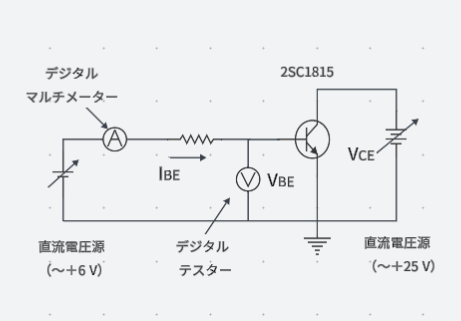
\includegraphics[width=0.8\linewidth]{IbVbezu.png}
    \caption{バイポーラトランジスタの $I_{B}$-$V_{BE}$静特性測定系の概略図}
    \label{fig:IbVbezu}
\end{figure}

\begin{figure}[H]
    \centering
    \includegraphics[width=0.8\linewidth]{npn1.png}
    \caption{配線図}
    \label{fig:npn1}
\end{figure}


npn形バイポーラトランジスタを用いて、$I_B$-$V_{BE}$静特性を測定した。
測定回路を作成し、$V_{CE}=0\,\mathrm{V}$および$V_{CE}=7.5\,\mathrm{V}$の場合について，
直流電源により$V_{BE}$を徐々に変化させた。
そのときのベース電流$I_B$をデジタルマルチメータで読み取り，$V_{BE}$と$I_B$の関係を記録した。

また，$V_{CE}=7.5\,\mathrm{V}$の場合の測定結果を用いて，
隣り合う測定点の差分から小信号入力インピーダンス$h_{ie}$を求めた。



\subsection{npn形バイポーラトランジスタの $I_{C}$-$V_{CE}$ 静特性測定}
図\ref{fig:IcVcezu}に測定系の概略図を示す。
また、図\ref{fig:npn2}に配線図を示す。

\begin{figure}[H]
    \centering
    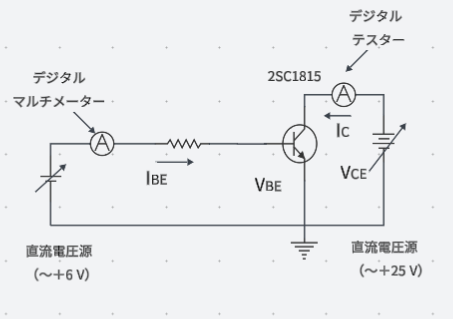
\includegraphics[width=0.8\linewidth]{IcVcezu.png}
    \caption{バイポーラトランジスタの $I_{C}$-$V_{CE}$静特性測定系の概略図}
    \label{fig:IcVcezu}
\end{figure}

\begin{figure}[H]
    \centering
    \includegraphics[width=0.8\linewidth]{npn2.png}
    \caption{配線図}
    \label{fig:npn2}
\end{figure}


ベース電流$I_B$を$5\,\mu\mathrm{A}$，$10\,\mu\mathrm{A}$，$15\,\mu\mathrm{A}$，
$20\,\mu\mathrm{A}$，$25\,\mu\mathrm{A}$，$30\,\mu\mathrm{A}$に設定し、
それぞれの場合について、$V_{CE}$を$0.1\,\mathrm{V}$から$15\,\mathrm{V}$まで変化させた。
そのときのコレクタ電流$I_C$をデジタルマルチメータで読み取り、
$V_{CE}$と$I_C$の関係を記録した。

さらに、$V_{CE}=7.5\,\mathrm{V}$における測定結果を用いて、
隣り合う測定点の差分から電流増幅率$h_{fe}$を求めた。


\section{結果}
\subsection{$I_B$-$V_{BE}$特性}

$V_{CE}=0~\mathrm{V}$および$7.5~\mathrm{V}$において測定した
$I_B$-$V_{BE}$特性を表\ref{tab:ibvbe0}および表\ref{tab:ibvbe75}に示す。
また，これらの測定結果をグラフ化したものを図\ref{fig:ibvbe}に示す。

\begin{table}[H]
\centering
\caption{$V_{CE}=0$ Vにおける$I_B-V_{BE}$特性}
\label{tab:ibvbe0
}
\begin{tabular}{cc}
\toprule
$V_{BE}$ [V] & $I_B$ [$\mu$A]\\
\midrule
0.445 & 1.0\\
0.467 & 1.9\\
0.483 & 3.0\\
0.493 & 4.0\\
0.502 & 5.0\\
0.511 & 6.1\\
0.517 & 7.1\\
0.523 & 8.0\\
0.529 & 9.1\\
0.533 & 10.1\\
0.538 & 11.1\\
0.541 & 12.0\\
0.545 & 13.0\\
0.549 & 14.0\\
0.552 & 15.0\\
0.565 & 20.0\\
0.574 & 25.0\\
0.582 & 30.0\\
0.588 & 35.1\\
0.593 & 40.1\\
0.597 & 45.0\\
0.602 & 50.0\\
0.605 & 55.0\\
\bottomrule
\end{tabular}
\end{table}

\begin{table}[H]
\centering
\caption{$V_{CE}=7.5$ Vにおける$I_B-V_{BE}$特性}
\label{tab:ibvbe75}
\begin{tabular}{cc}
\toprule
$V_{BE}$ [V] & $I_B$ [$\mu$A]\\
\midrule
0.500 & 0.1\\
0.605 & 1.1\\
0.622 & 2.0\\
0.632 & 3.0\\
0.640 & 4.0\\
0.646 & 5.0\\
0.650 & 6.0\\
0.654 & 7.0\\
0.657 & 8.0\\
0.661 & 9.0\\
0.663 & 10.0\\
0.665 & 11.0\\
0.667 & 12.0\\
0.669 & 13.0\\
0.671 & 14.1\\
0.672 & 15.0\\
0.679 & 20.1\\
0.684 & 25.0\\
0.688 & 30.0\\
0.691 & 35.1\\
0.690 & 40.0\\
0.684 & 45.0\\
0.680 & 50.0\\
\bottomrule
\end{tabular}
\end{table}

\begin{figure}[H]
    \centering
    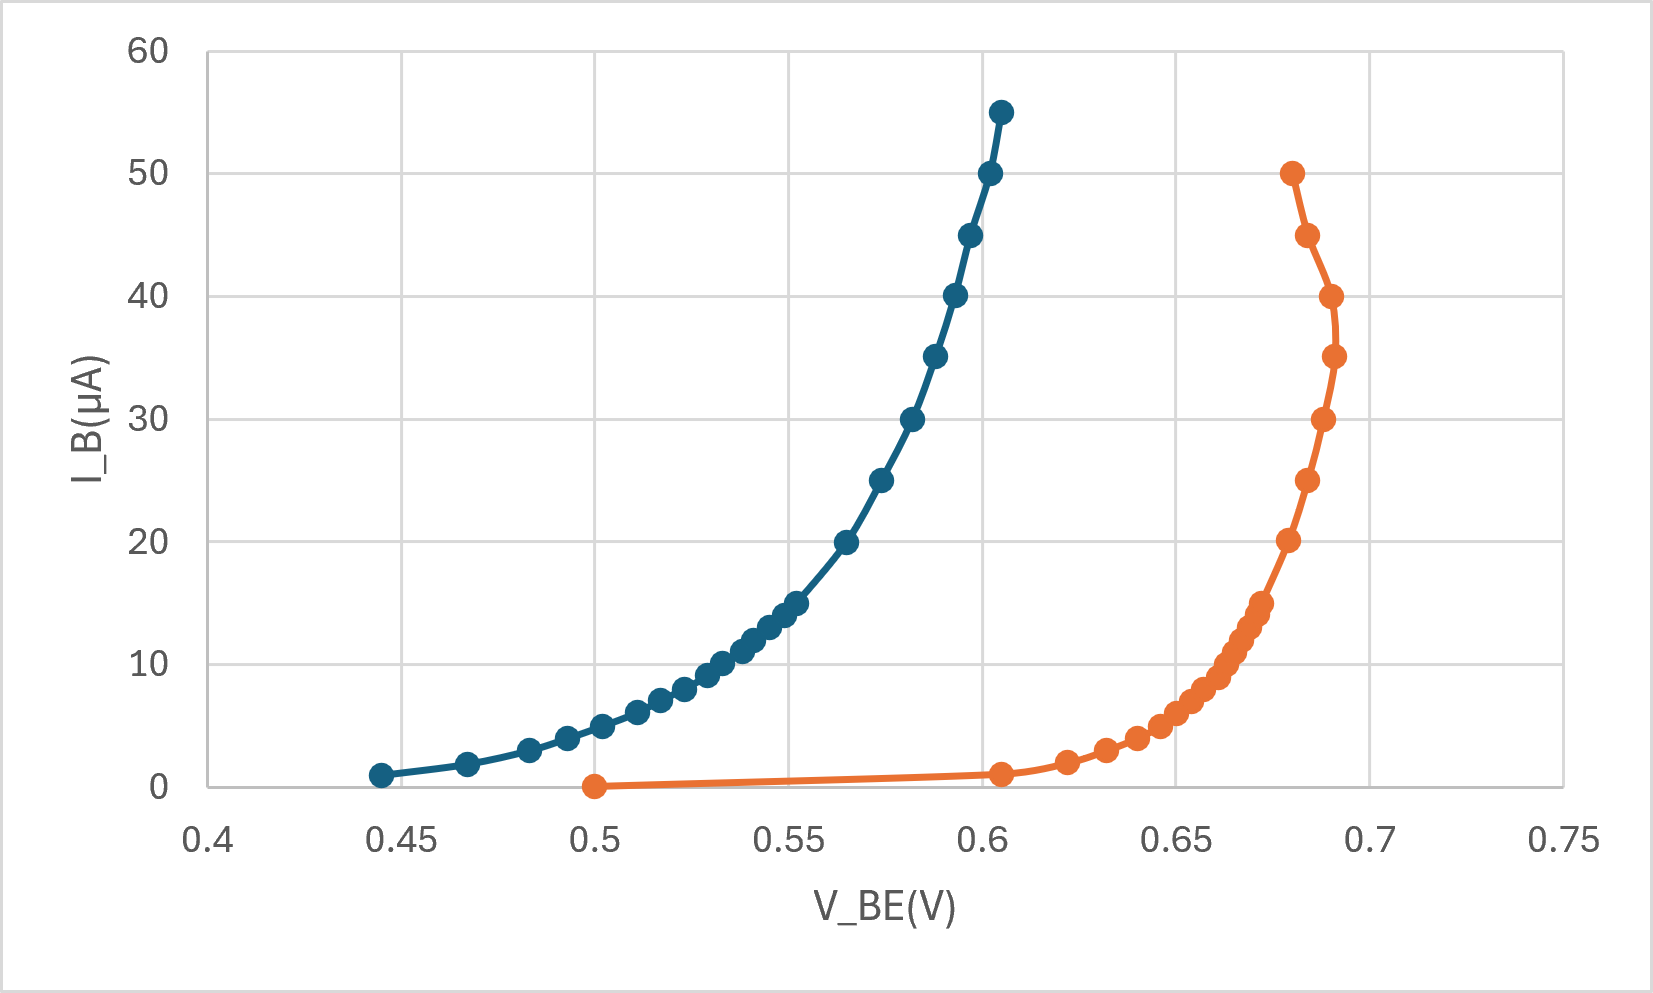
\includegraphics[width=0.8\linewidth]{vbe075.png}
    \caption{$V_{CE}=0~\mathrm{V}$および$7.5~\mathrm{V}$における$I_B$-$V_{BE}$特性}
    \label{fig:ibvbe}
\end{figure}

さらに，$V_{CE}=7.5~\mathrm{V}$における測定結果から，
隣接する測定点の差分を用いて小信号入力インピーダンス
$h_{ie}$を算出した。その結果を表\ref{tab:hie}および図\ref{fig:hiezu}に示す。
ただし、
縦軸の上限は$10\mathrm{k\Omega}$とし，それを越える点は省く。
\begin{table}[H]
\centering
\caption{$V_{CE}=7.5~\mathrm{V}$における$h_{ie}$の計算結果}
\label{tab:hie}
\begin{tabular}{cc}
\toprule
$V_{BE}$ [V] & $h_{ie}$ [$\Omega$] \\
\midrule
0.5525 & 105000 \\
0.6135 & 18888.9 \\
0.6270 & 10000 \\
0.6360 & 8000 \\
0.6430 & 6000 \\
0.6480 & 4000 \\
0.6520 & 4000 \\
0.6555 & 3000 \\
0.6590 & 4000 \\
0.6620 & 2000 \\
0.6640 & 2000 \\
0.6660 & 2000 \\
0.6680 & 2000 \\
0.6700 & 1818.2 \\
0.6715 & 1111.1 \\
0.6755 & 1372.5 \\
0.6815 & 1020.4 \\
0.6860 & 800.0 \\
0.6895 & 588.2 \\
0.6905 & -204.1 \\
0.6870 & -1200 \\
0.6820 & -800 \\
0.6800 & 13600 \\
\bottomrule
\end{tabular}
\end{table}

\begin{figure}[H]
    \centering
    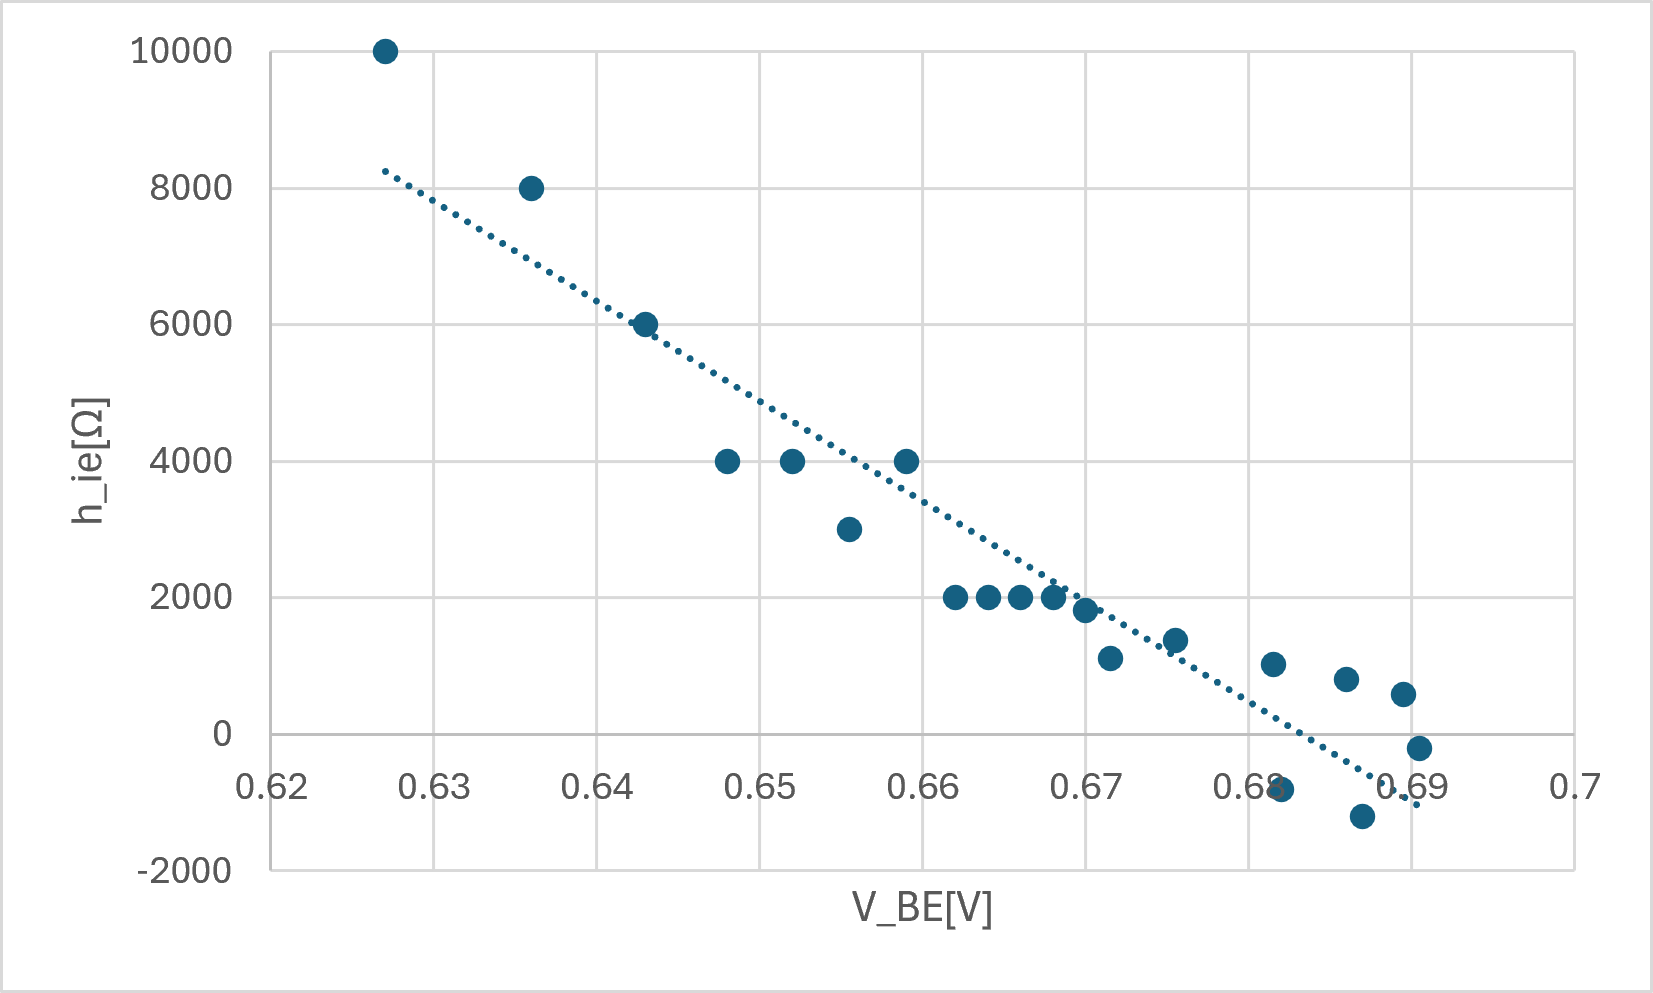
\includegraphics[width=0.8\linewidth]{hie.png}
    \caption{$V_{CE}=7.5~\mathrm{V}$における$h_{ie}$-$V_{BE}$特性}
    \label{fig:hiezu}
\end{figure}


\subsection{$I_C$-$V_{CE}$特性}

ベース電流$I_B$を5，10，15，20，25，30~$\mu$Aとした場合の
$I_C$-$V_{CE}$特性の測定結果を表\ref{tab:icvce}に示す。
また、測定結果をグラフ化したものを図\ref{fig:icvce}に示す。


\begin{table}[H]
\centering
\caption{$I_C$-$V_{CE}$特性の測定結果}
\label{tab:icvce}

\begin{minipage}{0.3\textwidth}
\centering
\small
\begin{tabular}{cc}
\toprule
\multicolumn{2}{c}{$I_B=5~\mu\mathrm{A}$}\\
\midrule
$V_{CE}$ [V] & $I_C$ [mA]\\
\midrule
0.1&0.42\\
0.2&0.64\\
0.3&0.64\\
1&0.65\\
2&0.65\\
3&0.65\\
5&0.66\\
7.5&0.66\\
9&0.66\\
12&0.67\\
15&0.67\\
\bottomrule
\end{tabular}
\end{minipage}
\hfill
\begin{minipage}{0.3\textwidth}
\centering
\small
\begin{tabular}{cc}
\toprule
\multicolumn{2}{c}{$I_B=10~\mu\mathrm{A}$}\\
\midrule
$V_{CE}$ [V] & $I_C$ [mA]\\
\midrule
0.1&0.82\\
0.2&1.31\\
0.3&1.32\\
0.4&1.32\\
0.6&1.32\\
1&1.33\\
2&1.33\\
4&1.34\\
6&1.35\\
7.5&1.35\\
9&1.36\\
12&1.37\\
15&1.38\\
\bottomrule
\end{tabular}
\end{minipage}
\hfill
\begin{minipage}{0.3\textwidth}
\centering
\small
\begin{tabular}{cc}
\toprule
\multicolumn{2}{c}{$I_B=15~\mu\mathrm{A}$}\\
\midrule
$V_{CE}$ [V] & $I_C$ [mA]\\
\midrule
0.1&0.59\\
0.2&1.99\\
0.3&2.00\\
0.4&2.00\\
0.6&2.00\\
1&2.00\\
3&2.02\\
5&2.04\\
7.5&2.05\\
10&2.07\\
12&2.08\\
15&2.09\\
\bottomrule
\end{tabular}
\end{minipage}

\vspace{5mm}

\begin{minipage}{0.3\textwidth}
\centering
\small
\begin{tabular}{cc}
\toprule
\multicolumn{2}{c}{$I_B=20~\mu\mathrm{A}$}\\
\midrule
$V_{CE}$ [V] & $I_C$ [mA]\\
\midrule
0.1&1.56\\
0.2&2.66\\
0.3&2.67\\
0.4&2.67\\
0.5&2.67\\
0.8&2.68\\
1&2.68\\
2&2.69\\
3&2.70\\
6&2.74\\
7.5&2.75\\
9&2.77\\
12&2.80\\
15&2.82\\
\bottomrule
\end{tabular}
\end{minipage}
\hfill
\begin{minipage}{0.3\textwidth}
\centering
\small
\begin{tabular}{cc}
\toprule
\multicolumn{2}{c}{$I_B=25~\mu\mathrm{A}$}\\
\midrule
$V_{CE}$ [V] & $I_C$ [mA]\\
\midrule
0.1&0.95\\
0.2&3.31\\
0.3&3.34\\
0.4&3.35\\
0.5&3.35\\
0.8&3.35\\
1&3.36\\
2&3.37\\
3&3.39\\
5&3.42\\
7.5&3.45\\
9&3.47\\
12&3.52\\
15&3.56\\
\bottomrule
\end{tabular}
\end{minipage}
\hfill
\begin{minipage}{0.3\textwidth}
\centering
\small
\begin{tabular}{cc}
\toprule
\multicolumn{2}{c}{$I_B=30~\mu\mathrm{A}$}\\
\midrule
$V_{CE}$ [V] & $I_C$ [mA]\\
\midrule
0.1&3.04\\
0.2&3.61\\
0.3&4.00\\
0.4&4.03\\
0.5&4.03\\
0.8&4.04\\
1&4.04\\
2&4.06\\
3&4.08\\
5&4.12\\
7.5&4.17\\
9&4.19\\
12&4.26\\
15&4.33\\
\bottomrule
\end{tabular}
\end{minipage}

\end{table}

図\ref{fig:icvce}における各曲線とベース電流との対応を表\ref{tab:graphcolor}に示す。
\begin{table}[H]
\centering
\caption{各曲線とベース電流との対応}
\label{tab:graphcolor}
\begin{tabular}{cc}
\toprule
$I_B$ [$\mu$A] & 色 \\
\midrule
5  & 赤 \\
10 & オレンジ \\
15 & 黒 \\
20 & 水色 \\
25 & 紫 \\
30 & 黄緑 \\
\bottomrule
\end{tabular}
\end{table}

\begin{figure}[H]
\centering
    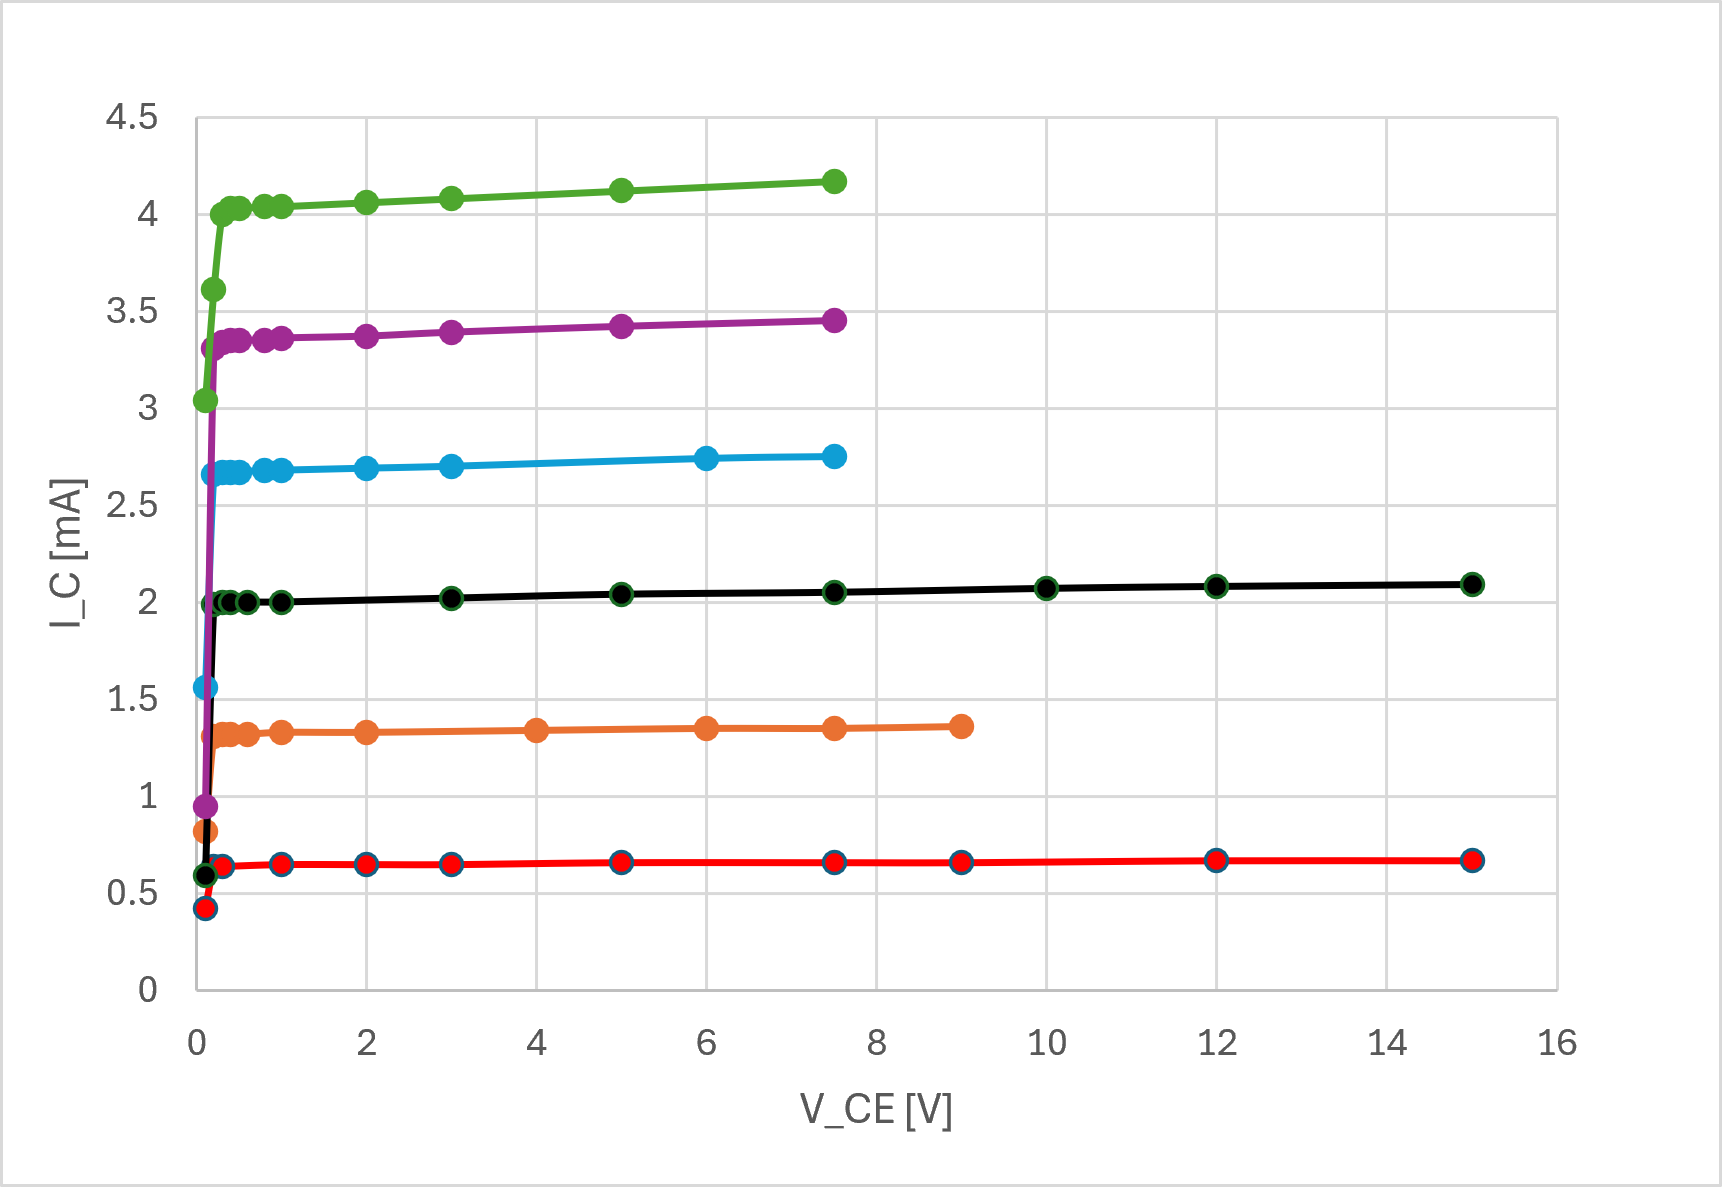
\includegraphics[width=0.8\linewidth]{icvce.png}
\caption{$I_C$-$V_{CE}$特性}
\label{fig:icvce}
\end{figure}



\section{考察}

\end{document}